\section{Results}
\label{sec:results}

Data and source code for analyses and plots are available in a Github repository at: \url{https://github.com/ew282d-evangelista/ew282d-sp2020-0451-trombetta}.

\subsection{Improvised force plate kymograph}
\Fref{fig:results:forceplate}A-B gives the force plate kymograph traces for two heel- versus toe-strike trials. Maximum vertical GRFs appear approximately equal in magnitude among the two treatments.  Some traces appear to show lateral movement of the force plate (yellow arrows); these appear to happen only in toe-strike trials, including an additional toe-strike trial to check for this effect (\fref{fig:results:forceplate}C). \Fref{fig:results:forceplate}C appears to show the lateral motion only occurs with the left foot. 
\begin{figure}
\begin{center}
%a \includegraphics[width=0.29\columnwidth]{figures/results3.png}
%b 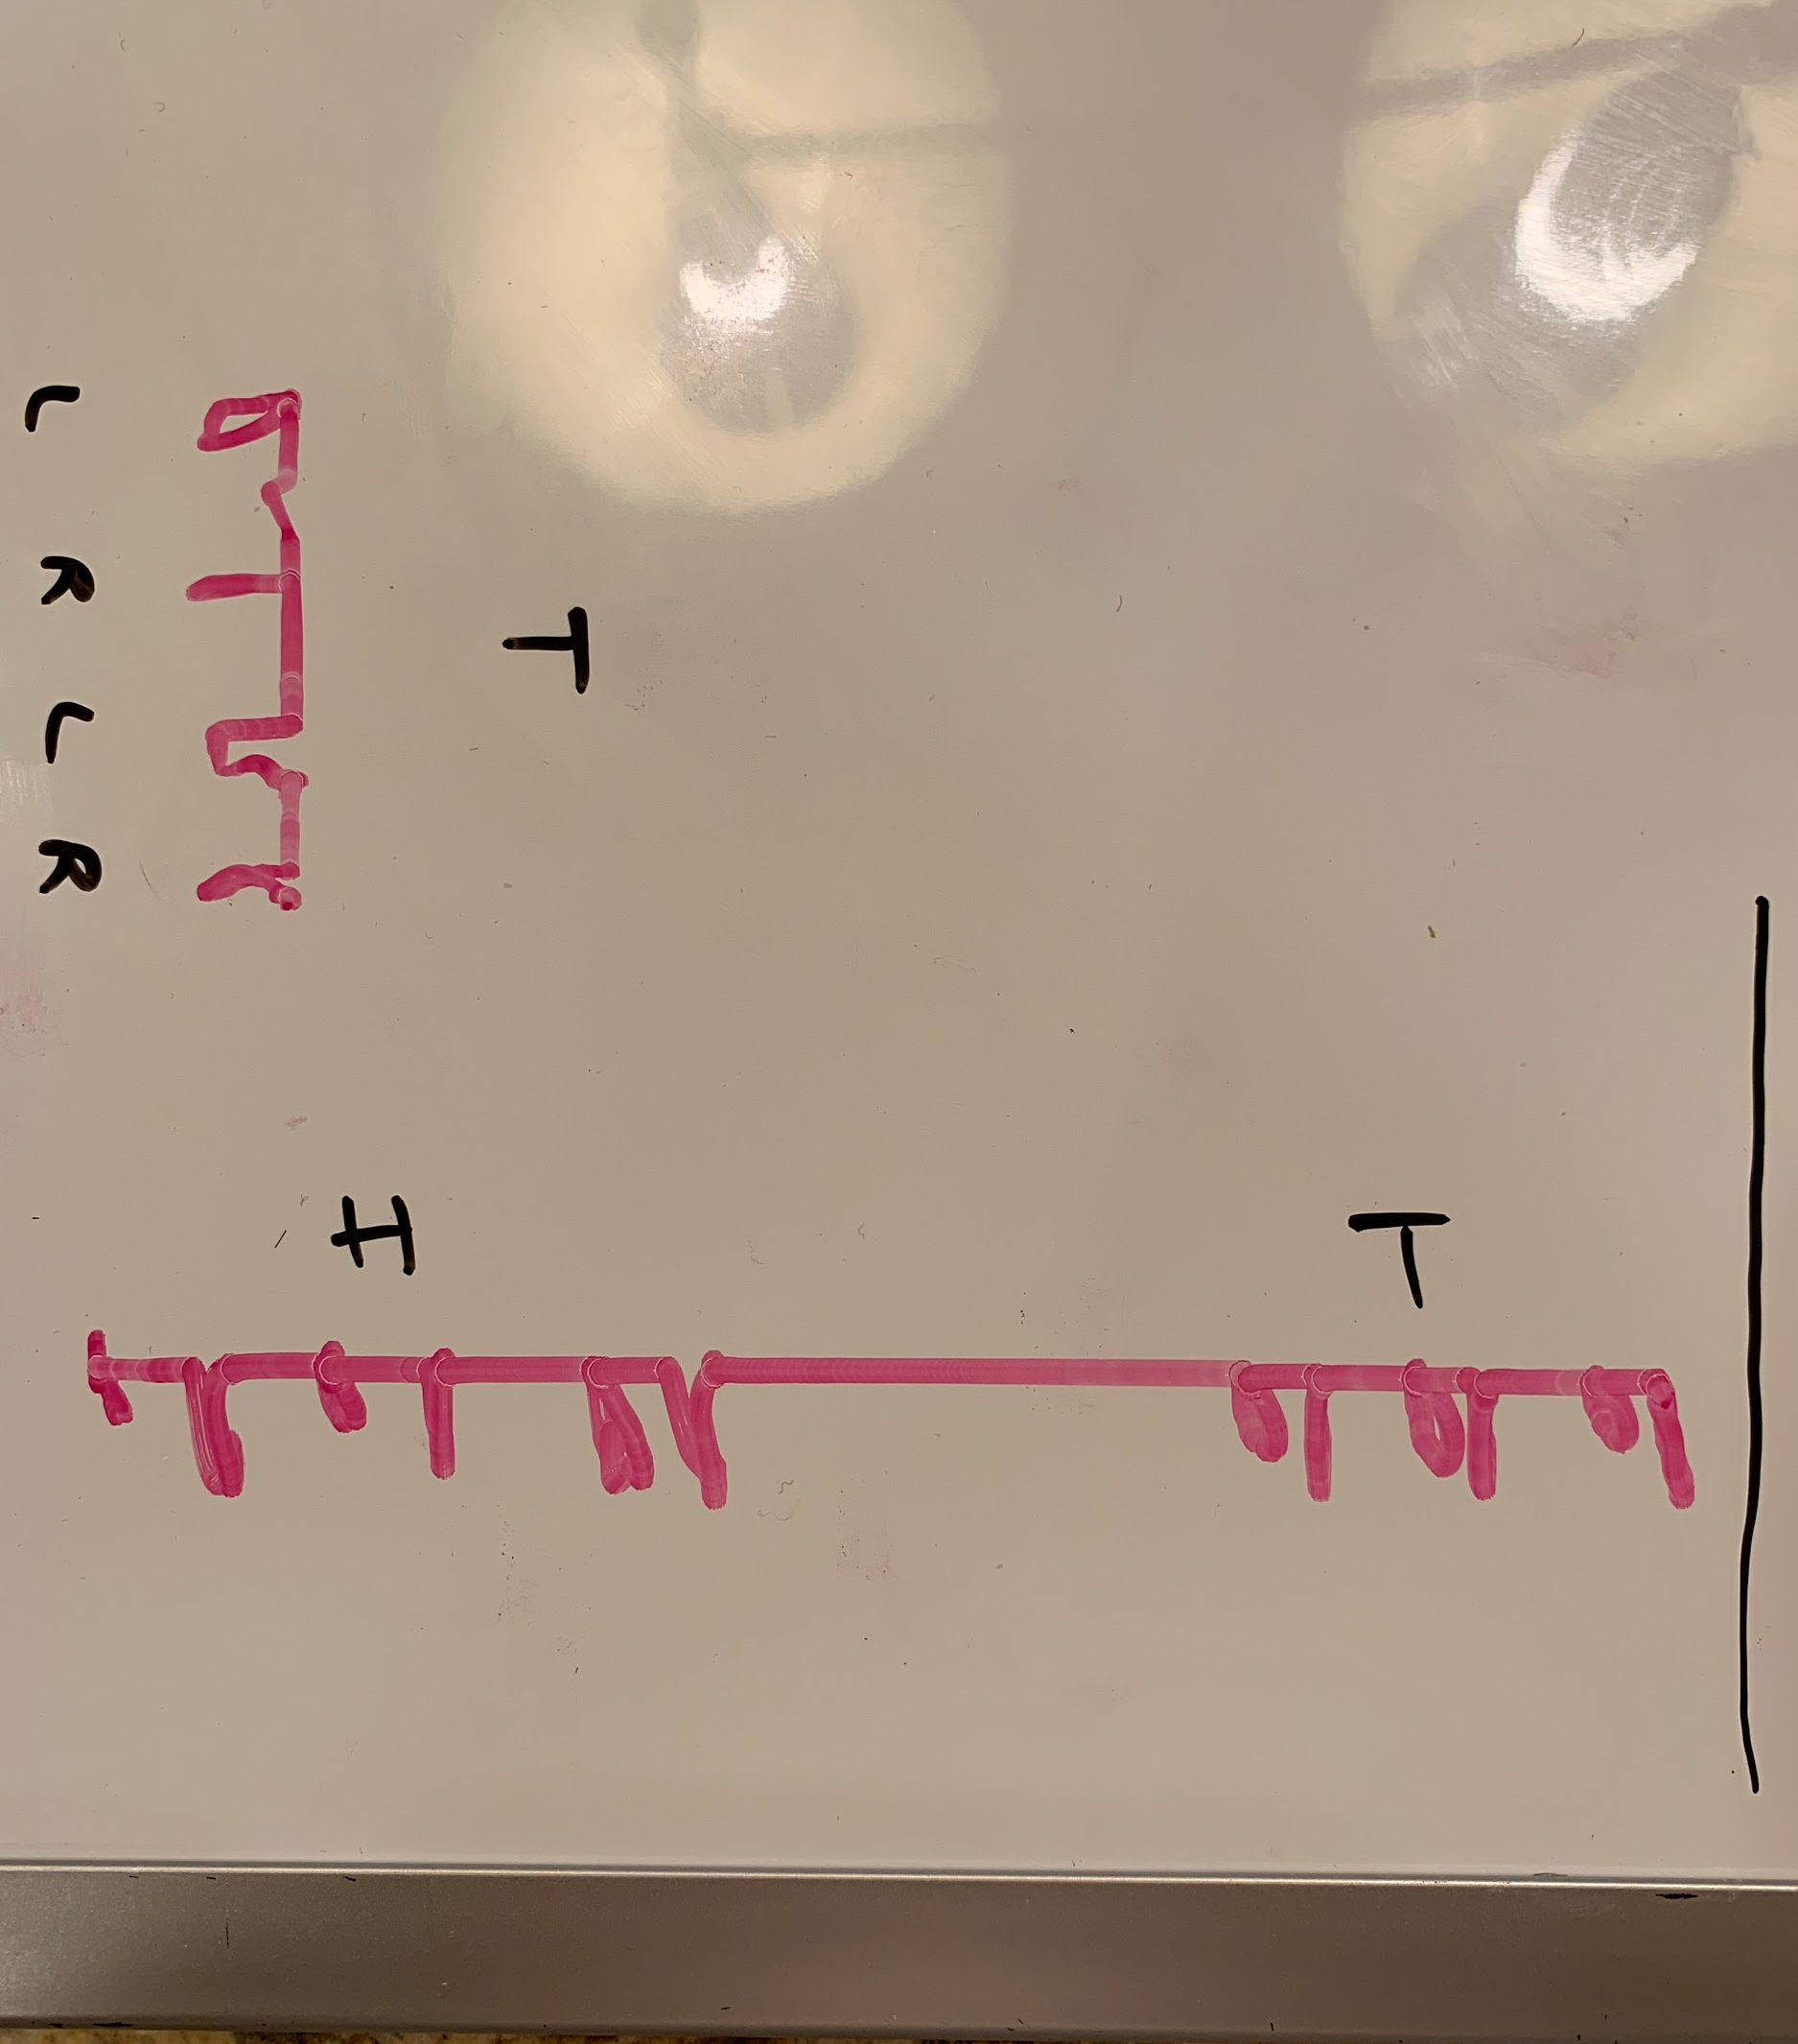
\includegraphics[width=0.29\columnwidth]{figures/results4.png}
%c 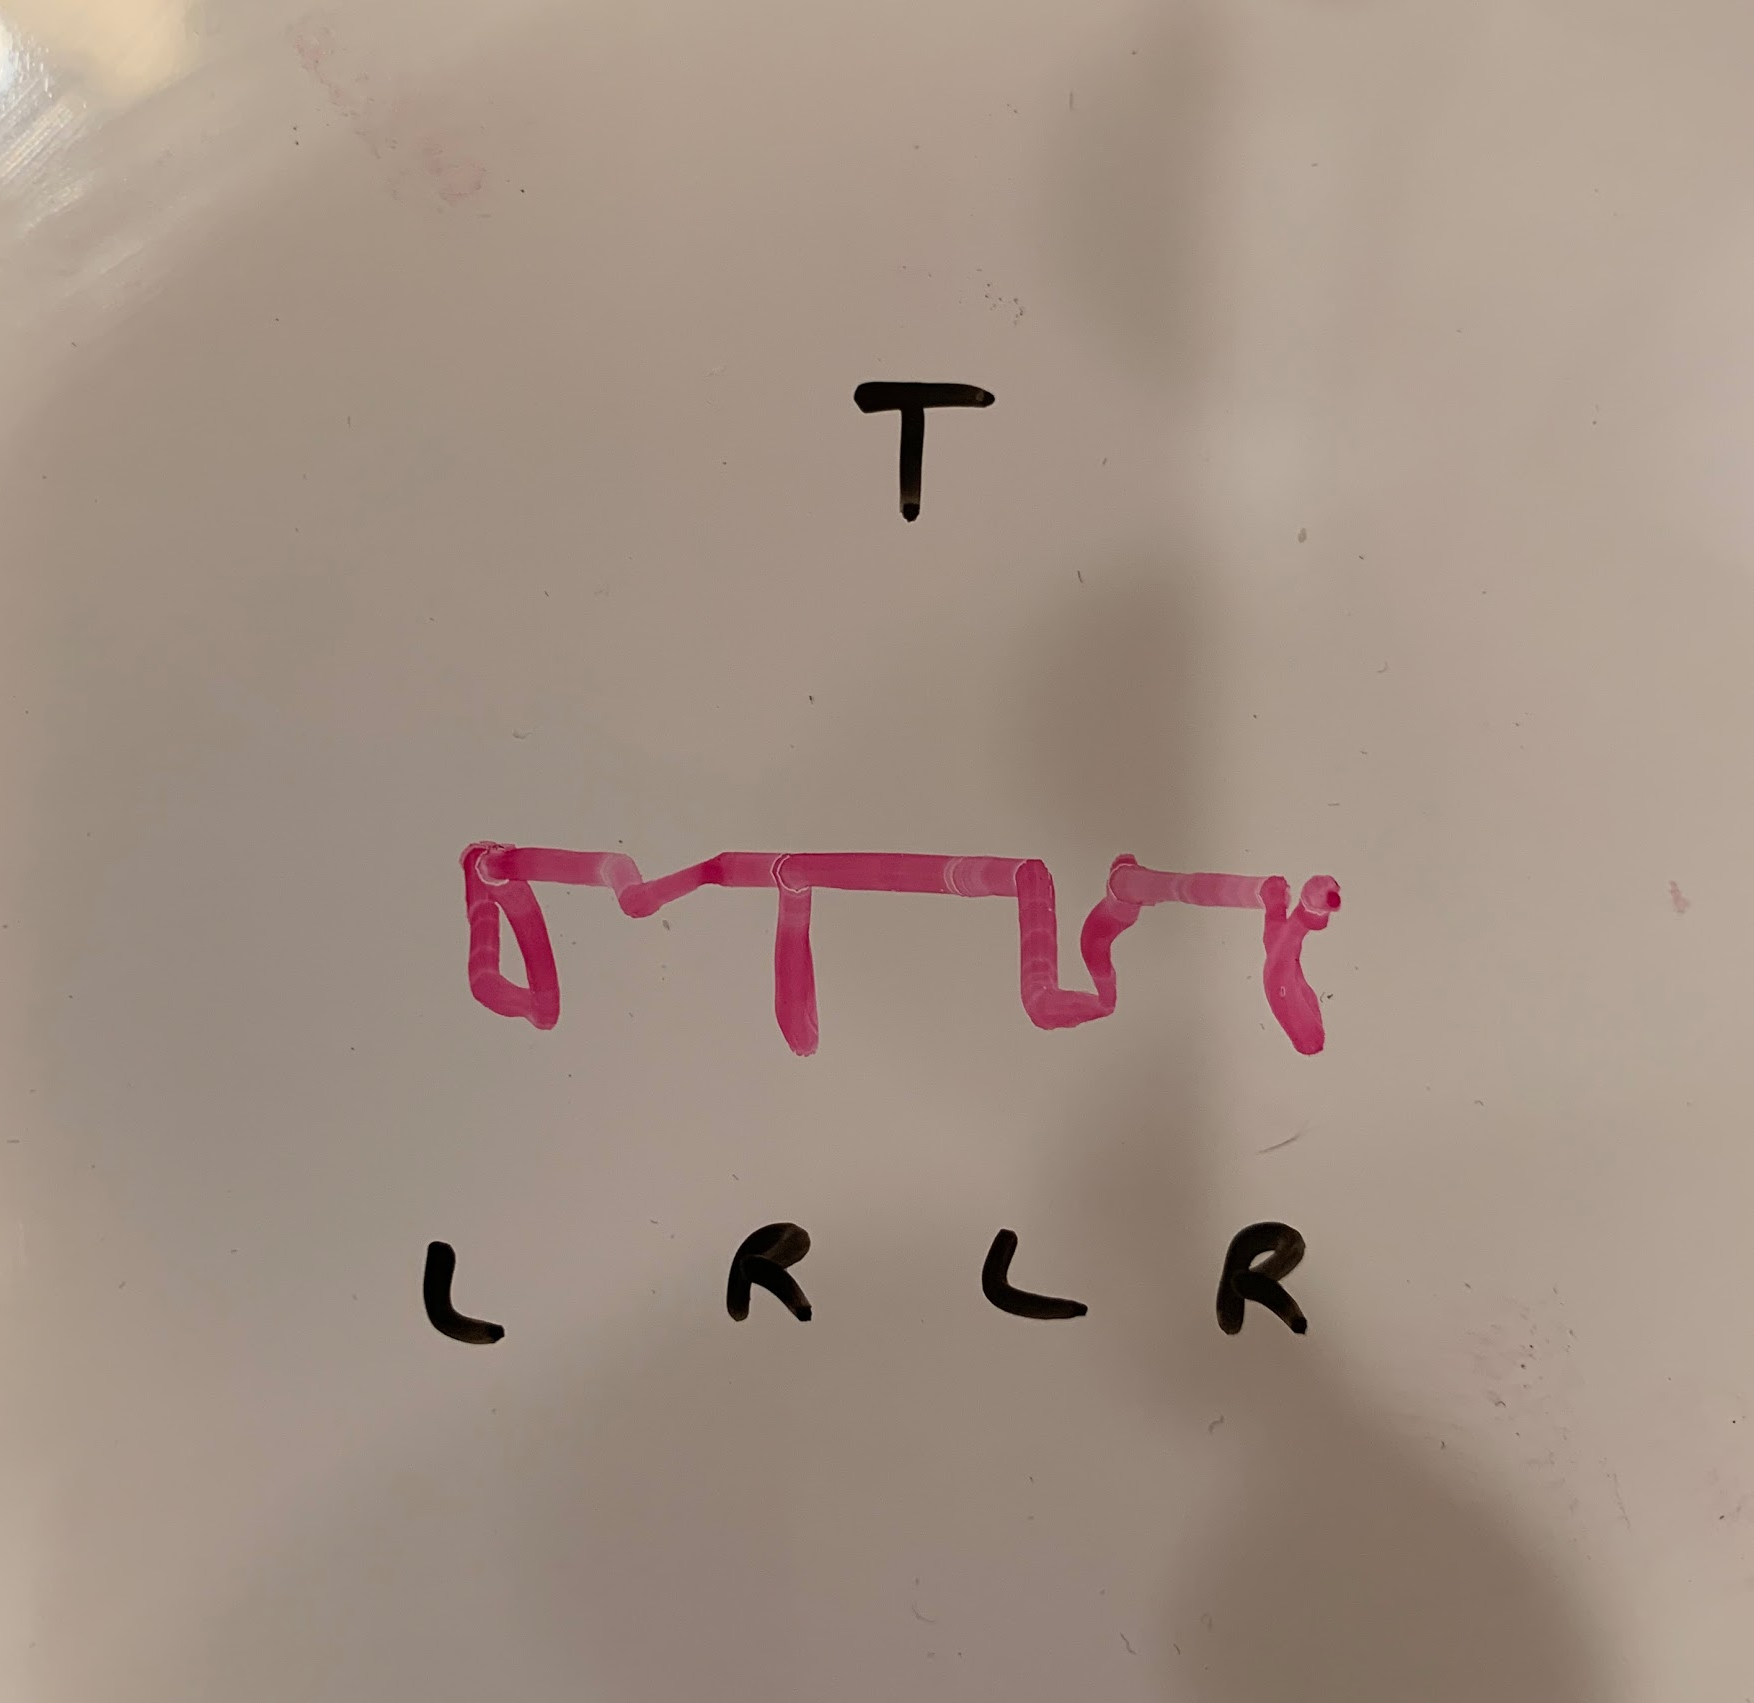
\includegraphics[width=0.29\columnwidth]{figures/results5.png}
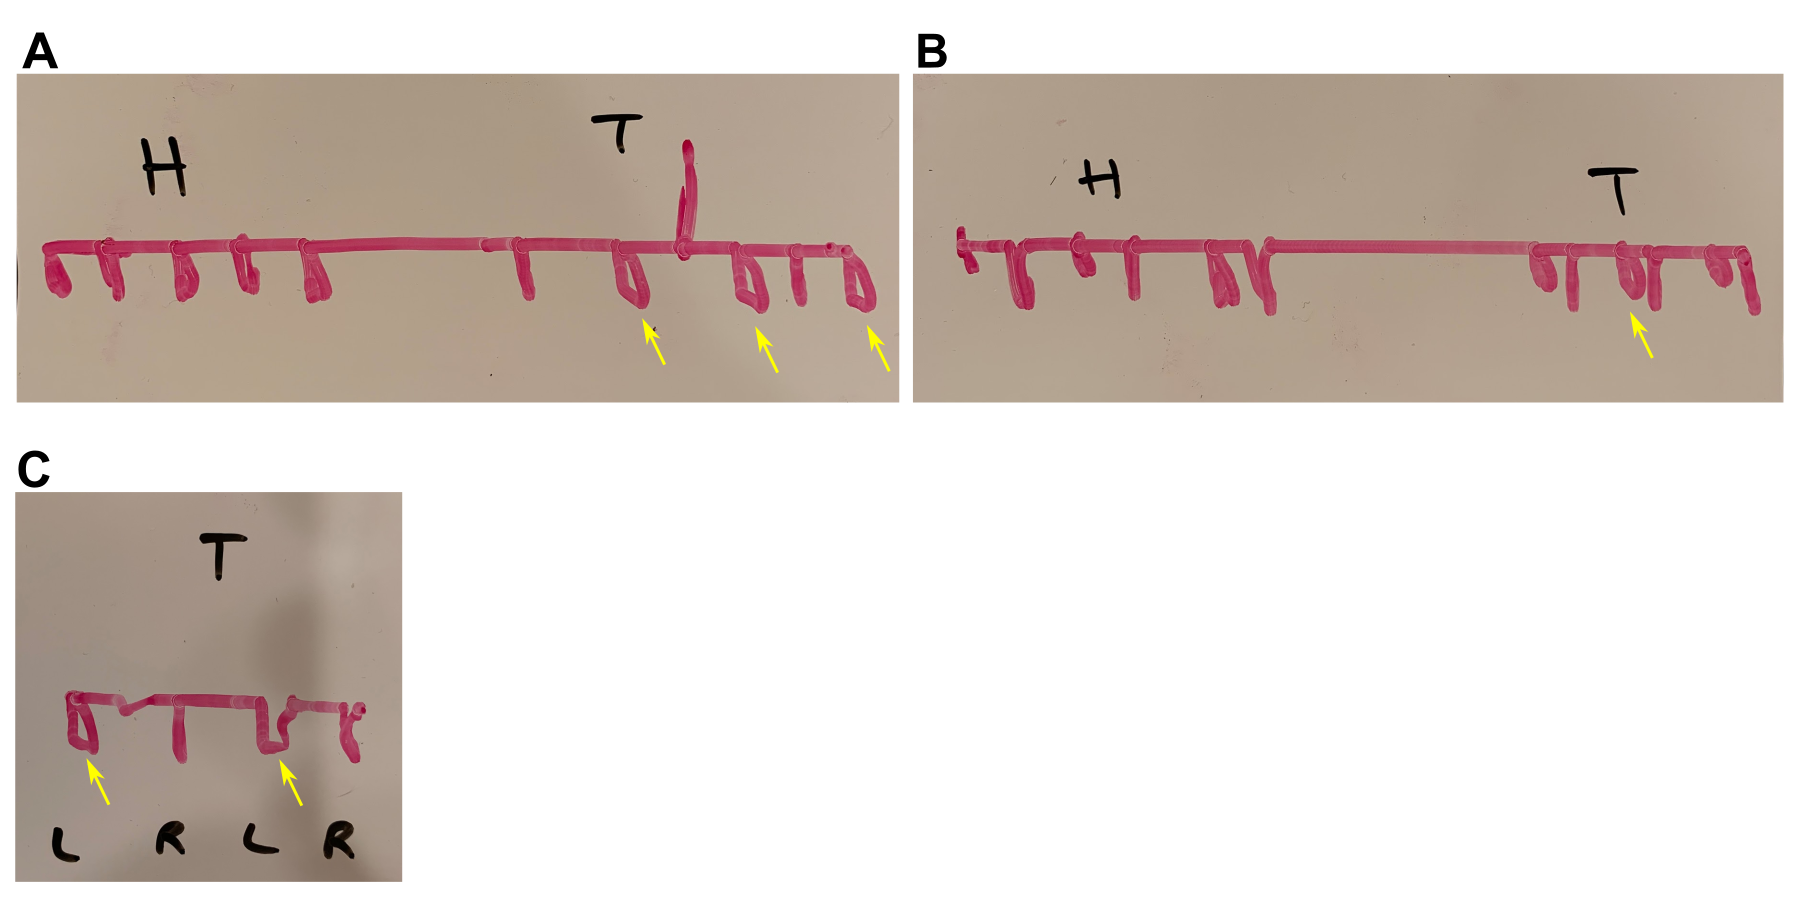
\includegraphics[width=0.75\columnwidth]{figures/fig-results-4.png}
\end{center}
\caption{Improvised force plate recordings of vertical ground reaction force; (A) and (B) trials comparing heel-strike (H) and toe-strike (T); (C) checking horizontal GRF toe-strike. Yellow arrows denote steps in which there appears to be either platform motion or a large horizontal GRF as evidenced by visible white within the center of the trace.}
\label{fig:results:forceplate}
\end{figure}





\subsection{Measurements of acceleration using a smartphone}
\SI{10}{\second} recordings of the vertical ($Y$) acceleration during running with heel- and toe-strike are shown in~\fref{fig:results:accel}. Toe-strike appears to provide slightly higher peaks accelerations, but is not statistically different from heel-strike (ANOVA, $p=0.551$, $n=1998$). Vertical accelerations (mean$\pm$s.d.) are \SI{9.5\pm8.8}{\meter\per\second\squared} for heel-strike and \SI{9.3\pm10}{\meter\per\second\squared} for toe-strike. 
\begin{figure}[h]
\begin{center}
%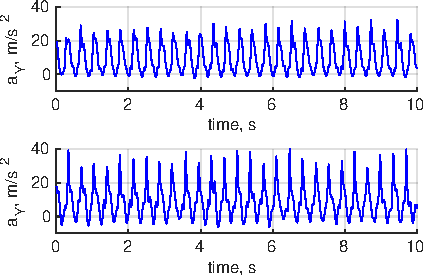
\includegraphics{data/accel/accelerations-raw.pdf}
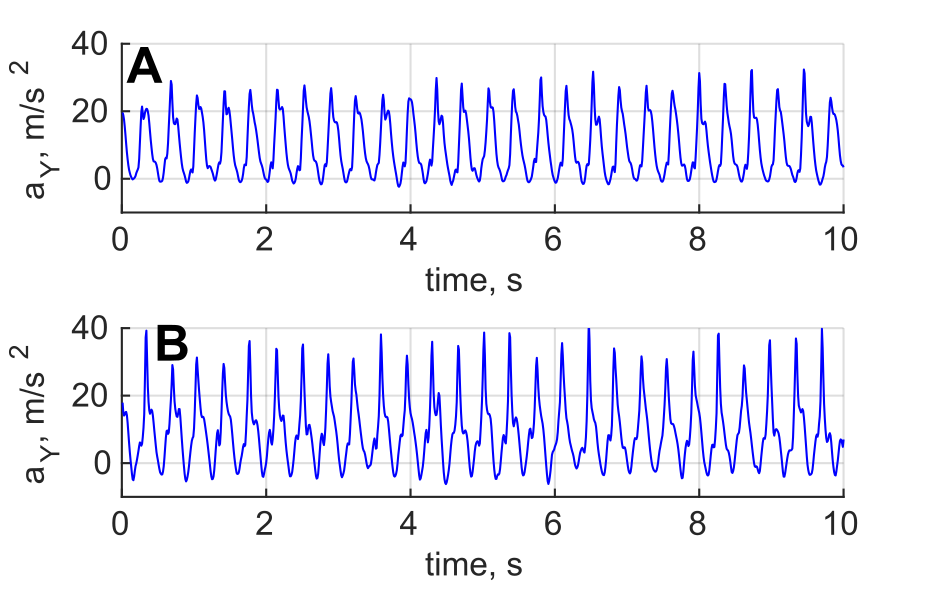
\includegraphics[width=3.1in]{figures/fig-results-5.png}
\end{center}
\caption{$Y$ (approximately vertical) accelerations recorded during running with (A) heel-strike and (B) toe-strike.}
\label{fig:results:accel}
\end{figure}





\subsection{Video kinematics on a treadmill}
Figures~\ref{fig:results:heelpretty} and \ref{fig:results:toepretty} show the digitized kinematics from running on the treadmill at \SI{8}{mph} (\SI{3.6}{\meter\per\second}). A \SI{1}{\meter} scale is provided at the bottom right. Heel- or foot-strike position is indicated with triangles, and the portions of the digitized leg positions in which the leg is in stance phase are shown in color. Directions are reversed from the original video recording to show conventional motion to the right. 
\begin{figure}[p]
\begin{center}
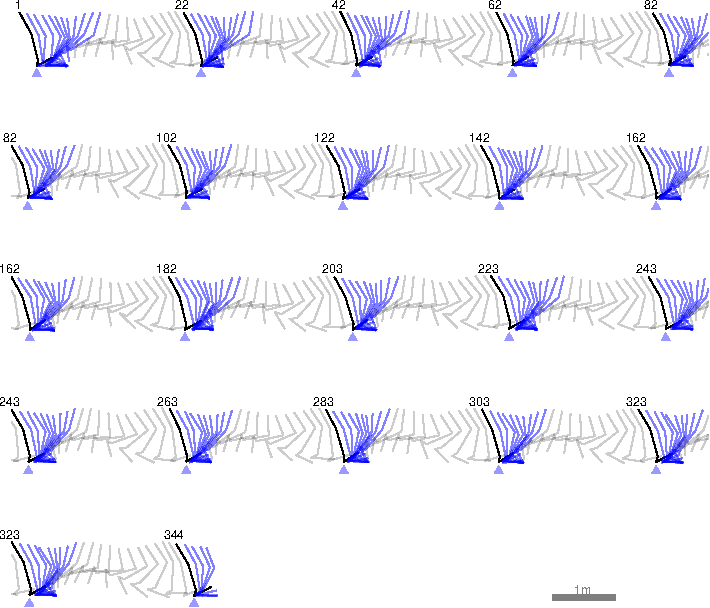
\includegraphics{data/heel-pretty.pdf}
\end{center}
\caption{Digitized kinematics from heel-strike running on a treadmill at \SI{8}{mph} (\SI{3.6}{\meter\per\second}). Heel strike position indicated with triangles. Stance phase for this leg indicated in blue. Numbers indicate video frame. Directions reversed from video. After \citep{marey1873locomotion, muybridge1901human}.}  
\label{fig:results:heelpretty}
\end{figure}

\begin{figure}[p]
\begin{center}
\includegraphics{data/toe-pretty.pdf}
\end{center}
\caption{Digitized kinematics from toe-strike running on a treadmill at \SI{8}{mph} (\SI{3.6}{\meter\per\second}). Toe strike position indicated with triangles. Stance phase for this leg indicated in red. Numbers indicate video frame. Directions reversed from video. After \citep{marey1873locomotion, muybridge1901human}.}  
\label{fig:results:toepretty}
\end{figure}

The reduced data for 17 heel-strike and 21 toe-strike steps are shown in \fref{fig:results:stride} and \fref{tab:results:stride}. Results show statistically significant differences: toe-strike stride period is shorter (ANOVA, $p=\num{4.7e-7}$, $n=17$), stride frequency is higher (ANOVA, $p=\num{5e-7}$), stride length is shorter (ANOVA, $p=\num{4.7e-7}$), and duty cycle is shorter (ANOVA, $p=\num{3e-10}$).
\begin{figure}
\begin{center}
\includegraphics{figures/stride-data.png}
\end{center}
\caption{Reduced stride data for 17 heel-strike and 21 toe-strike steps during running on a treadmill at \SI{8}{mph} (\SI{3.6}{\meter\per\second}), including (a) stride period; (b) stride frequency, (c) stride length and (d) duty cycle. Stastically significant differences marked; toe-strike stride period is shorter (ANOVA, $p=\num{4.7e-7}$, $n=17$), stride frequency is higher (ANOVA, $p=\num{5e-7}$), stride length is shorter (ANOVA, $p=\num{4.7e-7}$), and duty cycle is shorter (ANOVA, $p=\num{3e-10}$). See \fref{tab:results:stride}.} 
\label{fig:results:stride}
\end{figure}

\begin{table}[h]
\caption{Reduced stride data (mean$\pm$s.d.) for 17 heel-strike and 21 toe-strike steps during running on a treadmill. Toe-strike stride period is shorter (ANOVA, $p=\num{4.7e-7}$, $n=17$), stride frequency is higher (ANOVA, $p=\num{5e-7}$), stride length is shorter (ANOVA, $p=\num{4.7e-7}$), and duty cycle is shorter (ANOVA, $p=\num{3e-10}$). See \fref{fig:results:stride}.}
\label{tab:results:stride}
\begin{center}
\begin{tabular}{lcc}
\toprule
& heel-strike ($n=17$) & toe-strike ($n=21$)\\
\midrule 
stride period, \si{\second}   & \num{0.67\pm0.01} & \num{0.64\pm0.02} \\
stride frequency, \si{\hertz} & \num{1.49\pm0.03} & \num{1.56\pm0.04} \\
stride length, \si{\meter}    & \num{2.41\pm0.05} & \num{2.29\pm0.06} \\
duty cycle                    & \num{0.46\pm0.03} & \num{0.40\pm0.02} \\
\bottomrule
\end{tabular}
\end{center}
\end{table}

Joint angle data for the foot, knee, and hip under heel-strike and toe-strike are shown in \fref{fig:results:jointangles}. \Fref{fig:results:jointangles} collapses all 17 (heel-strike) or 21 (toe-strike) steps into a single plot over one cycle of locomotion using the recovered phase \citep{revzen2008estimating}. Knee and hip angles appear similar between the two running styles, but foot angle shows clear differences immediately before and after foot contact with the ground. In heel-strike, the heel strikes with the foot dorsiflexed; while in toe-strike, the toe strikes the ground while the foot is plantar flexed.
\begin{figure}
\begin{center}
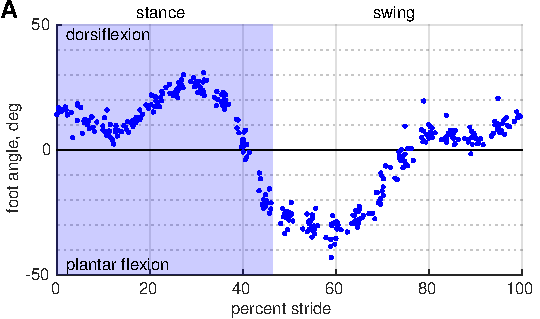
\includegraphics[width=0.49\columnwidth]{data/heel-foot-angle.pdf}
\includegraphics[width=0.49\columnwidth]{data/toe-foot-angle.pdf}\\
\includegraphics[width=0.49\columnwidth]{data/heel-knee-angle.pdf}
\includegraphics[width=0.49\columnwidth]{data/toe-knee-angle.pdf}\\
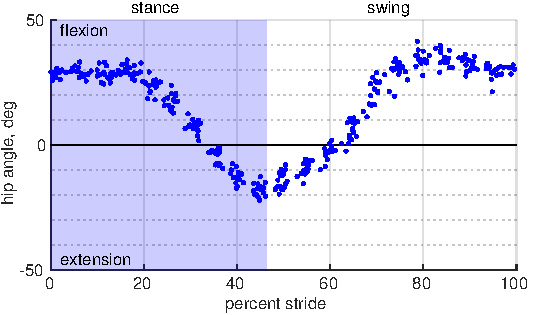
\includegraphics[width=0.49\columnwidth]{data/heel-hip-angle.pdf}
\includegraphics[width=0.49\columnwidth]{data/toe-hip-angle.pdf}
\end{center}
\caption{Joint angles for heel-strike and toe-strike running on a treadmill at \SI{8}{mph} (\SI{3.6}{\meter\per\second}). (A,B) Foot angle ($\alpha$); (C,D) knee angle ($\beta$); (E,F) hip angle ($\gamma$). Knee and hip angles appear similar between the two running styles, but foot angle shows clear differences immediately before and after foot contact with the ground. In heel-strike, the heel strikes with the foot dorsiflexed; while in toe-strike, the toe strikes the ground while the foot is plantar flexed, allowing it to act as a shock absorber.}
\label{fig:results:jointangles}
\end{figure}

\Fref{fig:results:contactangles} shows a comparison between the angle of the ankle and the contact angle, i.e. from the heel or toe to the hip. The angular misalignment between the ankle and the angle from the point of contact to the hip is \ang{3.3\pm0.8} in the case of heel-strike, and \ang{27.8\pm3.2} in the case of toe-strike. The difference between the two treatments is significant (Welch two sample t-test, $t=-34.358$, $df=24.476$, $p<\num{2.2e-16}$).
\begin{figure}
\begin{center}
\includegraphics{data/contact-angle.pdf}
\end{center}
\caption{Comparison of the angle of the ankle and the contact angle, from the heel or toe to the hip. In the case of heel-strike, the ankle and shins are well aligned with the contact angle with the ground (right). For toe-strike, the ankle and shins are not well aligned with the contact angle with the ground (left). The angular misalignment between the ankle and the angle from the point of contact to the hip is \ang{3.3\pm0.8} in the case of heel-strike, and \ang{27.8\pm3.2} in the case of toe-strike. The difference between the two treatments is significant (Welch two sample t-test, $t=-34.358$, $df=24.476$, $p<\num{2.2e-16}$).} 
\label{fig:results:contactangles}
\end{figure}
